\chapter{Results}
\label{cha:results}

\section{Example Analysis - the `top` process}

\begin{figure}
    \centering
    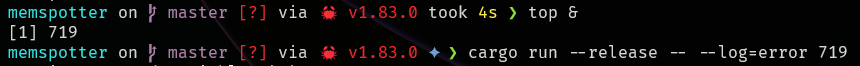
\includegraphics[width=0.5\linewidth]{cli-run.png}
    \caption{Caption}
    \label{fig:enter-label}
\end{figure}

\subsection{Brief UI overview}

\begin{figure}
    \centering
    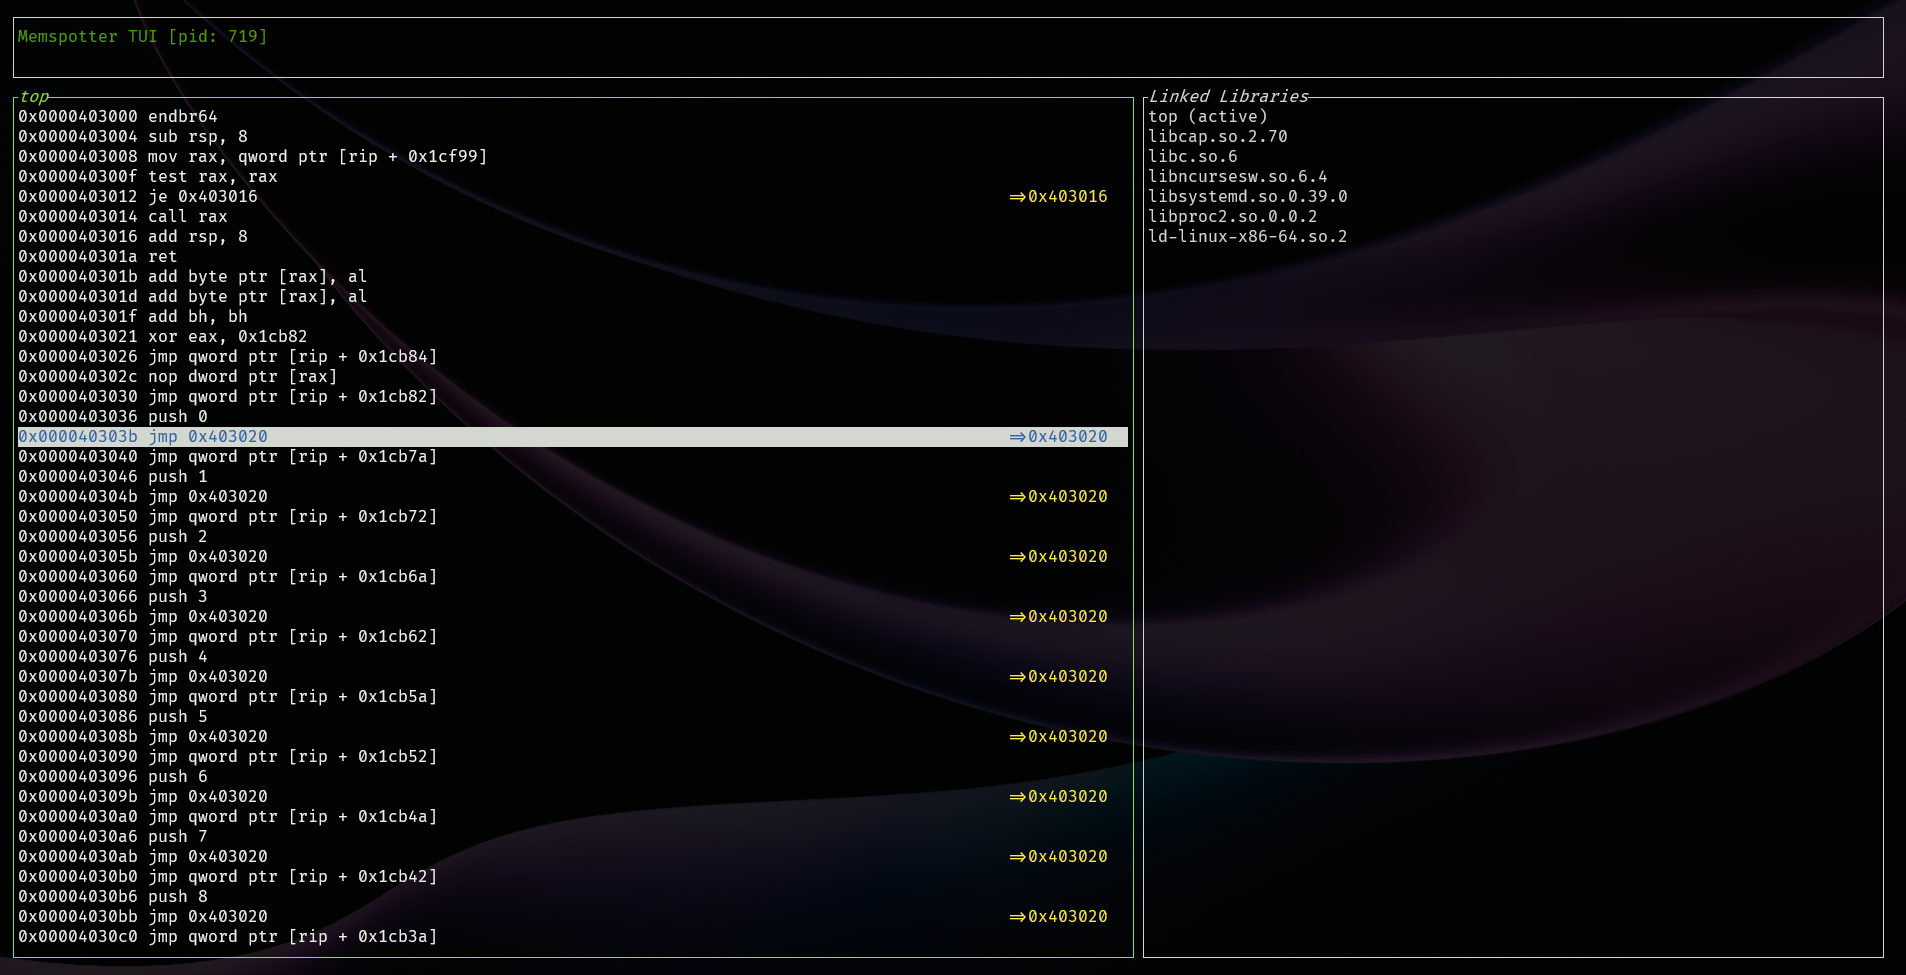
\includegraphics[width=0.5\linewidth]{tui-main.png}
    \caption{Caption}
    \label{fig:enter-label}
\end{figure}

\subsection{Analyzing the main library}

\begin{figure}
    \centering
    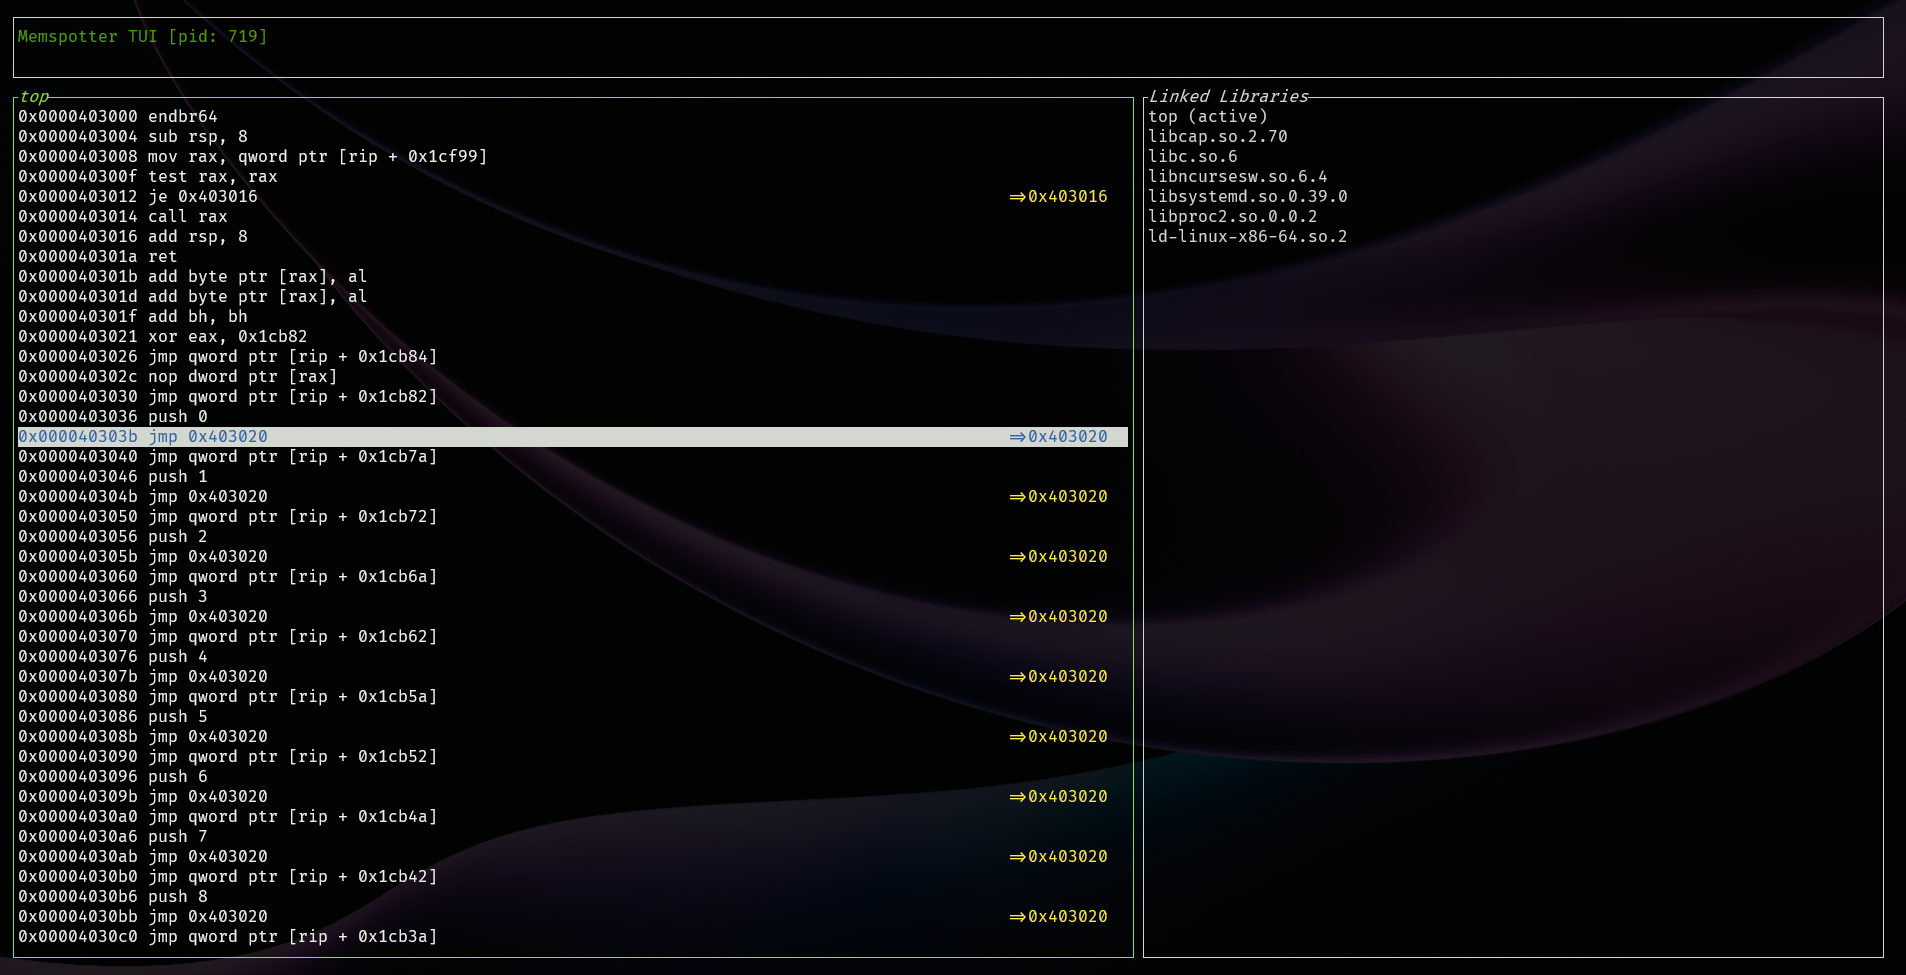
\includegraphics[width=0.5\linewidth]{tui-main.png}
    \caption{Caption}
    \label{fig:enter-label}
\end{figure}

\subsection{Main function and its calls}

\begin{figure}
    \centering
    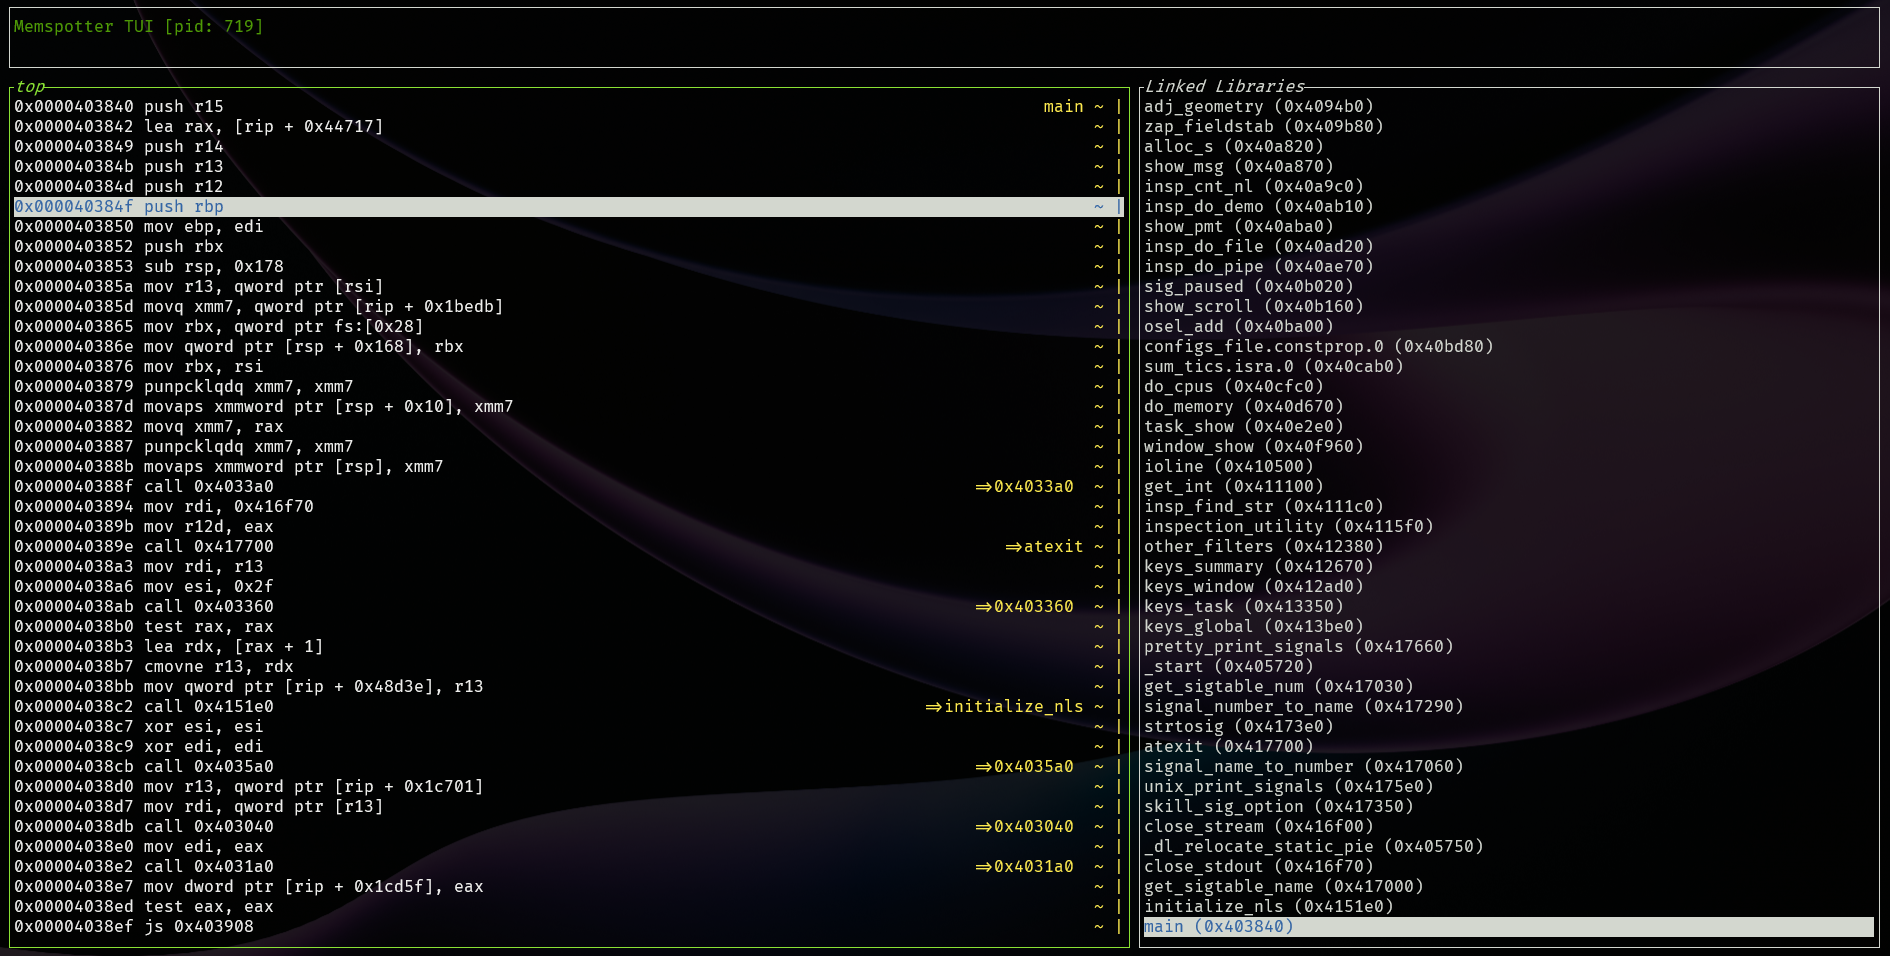
\includegraphics[width=0.5\linewidth]{tui-function-select.png}
    \caption{Caption}
    \label{fig:enter-label}
\end{figure}

\subsection{Brief look at dependencies}

\begin{figure}
    \centering
    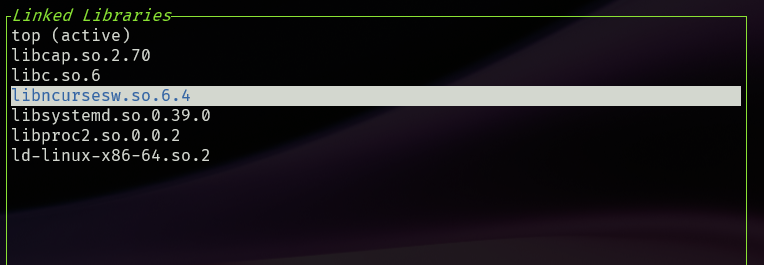
\includegraphics[width=0.5\linewidth]{tui-lib-select.png}
    \caption{Caption}
    \label{fig:enter-label}
\end{figure}

\subsection{Looking at compiler/linker optimizations and it's possible effects}

\begin{figure}
    \centering
    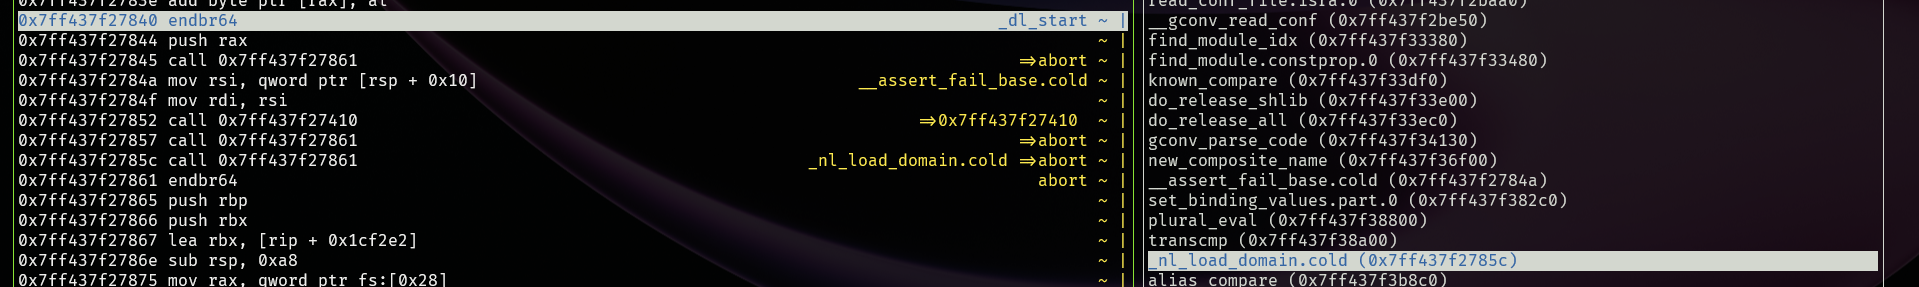
\includegraphics[width=0.5\linewidth]{cold-starts.png}
    \caption{Caption}
    \label{fig:enter-label}
\end{figure}

\begin{figure}
    \centering
    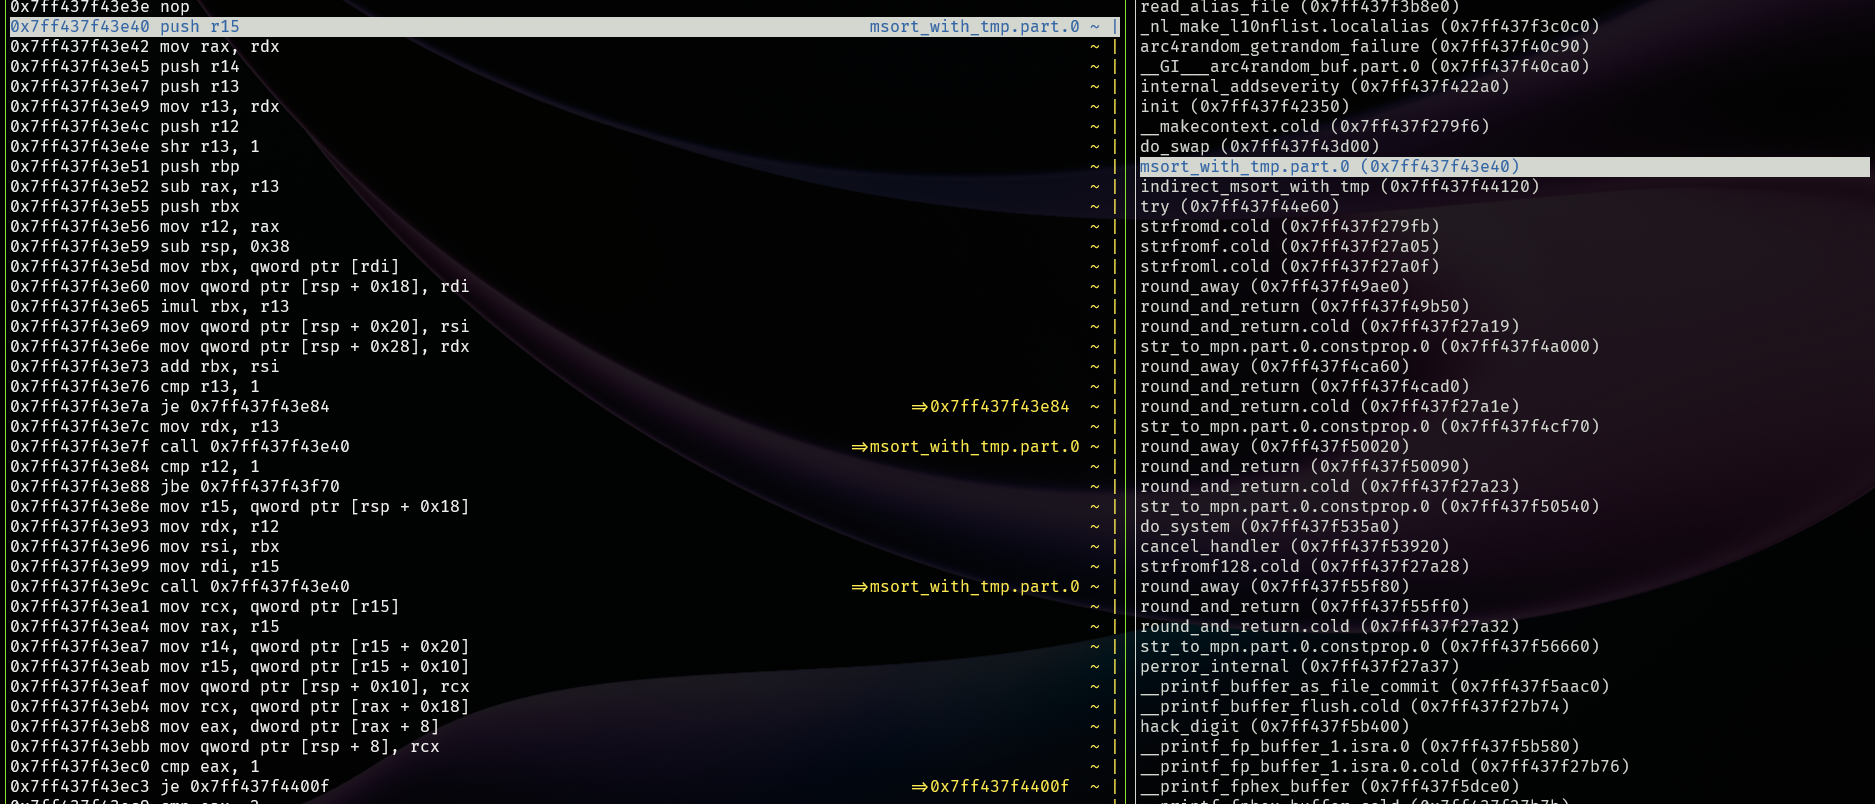
\includegraphics[width=0.5\linewidth]{function-parts.png}
    \caption{Caption}
    \label{fig:enter-label}
\end{figure}

Arch + SIMD
\begin{figure}
    \centering
    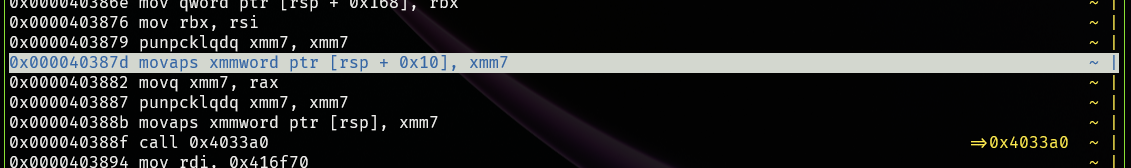
\includegraphics[width=0.5\linewidth]{arch-specific-instruction.png}
    \caption{Caption}
    \label{fig:enter-label}
\end{figure}